\section{Zpracování textových dat. Lingvistické zpracování přirozeného jazyka, jazykové modely, analytické metody, existující nástroje}

\subsection{Základní vymezení}

Zpracování textových dat se zabývá převodem textu do podoby, se kterou mohou pracovat analytické algoritmy.
Text jako takový je pro počítač pouze posloupnost znaků. Analytický model ale potřebuje příznaky:
\[
\text{text}
\rightarrow
\text{tokeny}
\rightarrow
\text{features / vectors}
\rightarrow
\text{model}.
\]

\textbf{Natural Language Processing} neboli NLP je oblast na pomezí lingvistiky, informatiky a umělé
inteligence, která se zabývá zpracováním přirozeného jazyka počítačem.

\textbf{Text analytics} lze chápat jako propojení NLP a datové analytiky nad texty. NLP často řeší jazykové
předzpracování a reprezentaci textu, zatímco text analytics se soustředí na získání analytického výstupu:
klasifikace, vyhledávání, sentiment, extrakce informací, sumarizace, topic modeling apod.

\paragraph{Příklad.}
Věta:
\begin{quote}
\uv{Zákazník si stěžoval na pomalé doručení.}
\end{quote}
může být převedena na:
\begin{itemize}
    \item tokeny: \texttt{Zákazník, si, stěžoval, na, pomalé, doručení};
    \item lemma: \texttt{zákazník, se, stěžovat, na, pomalý, doručení};
    \item sentiment: negativní;
    \item aspekt: doručení;
    \item entita: zákazník.
\end{itemize}

\subsection{Text není úplně bez struktury}

Text se často označuje jako nestrukturovaný, ale přirozený jazyk má mnoho vrstev:
\begin{itemize}
    \item znaky,
    \item morfémy,
    \item subword jednotky,
    \item slova,
    \item fráze,
    \item věty,
    \item odstavce,
    \item dokumenty.
\end{itemize}

Kromě toho má jazyk:
\begin{itemize}
    \item pravopis,
    \item gramatiku,
    \item morfologii,
    \item syntax,
    \item význam,
    \item pragmatiku a kontext.
\end{itemize}

\paragraph{Důležité pro češtinu.}
Čeština má bohatou morfologii a volnější slovosled než angličtina. Proto postupy vyvinuté pro angličtinu
nemusí bez úprav fungovat stejně dobře pro češtinu. U češtiny je důležitá hlavně kvalitní tokenizace,
lemmatizace a morfologické značkování.

\subsection{Obecný pipeline zpracování textu}

Typický postup:
\begin{enumerate}
    \item získání dokumentů,
    \item čištění textu,
    \item tokenizace,
    \item rozdělení na věty,
    \item normalizace,
    \item odstranění stop slov,
    \item stemming nebo lemmatizace,
    \item POS tagging a morfologická analýza,
    \item syntaktické zpracování,
    \item extrakce entit a vztahů,
    \item vytvoření číselné reprezentace,
    \item modelování a vyhodnocení.
\end{enumerate}

Ne všechny kroky jsou vždy potřeba. U moderních transformerových modelů se část jazykového zpracování učí
uvnitř modelu, ale porozumění těmto krokům je pořád důležité pro diagnostiku chyb a interpretaci výsledků.

\subsection{Čištění a normalizace textu}

Čištění textu zahrnuje:
\begin{itemize}
    \item odstranění HTML značek,
    \item odstranění boilerplate textu z webu,
    \item dekódování HTML entit,
    \item sjednocení kódování,
    \item odstranění duplicit,
    \item opravy typografických znaků,
    \item normalizaci mezer,
    \item zachování nebo odstranění interpunkce podle úlohy.
\end{itemize}

Normalizace může zahrnovat:
\begin{itemize}
    \item převod na malá písmena,
    \item normalizaci čísel,
    \item normalizaci URL adres,
    \item normalizaci uživatelských jmen,
    \item převod emotikonů,
    \item opravu překlepů.
\end{itemize}

\paragraph{Pozor.}
Převod na malá písmena může zhoršit NER, protože velká písmena pomáhají poznat jména osob, organizací a míst.

\subsection{Tokenizace}

Tokenizace rozděluje text na tokeny:
\[
\text{text}
\rightarrow
(t_1,t_2,\ldots,t_n).
\]

Token může být:
\begin{itemize}
    \item slovo,
    \item číslo,
    \item interpunkce,
    \item emotikon,
    \item subword jednotka,
    \item znak.
\end{itemize}

Příklad:
\begin{quote}
\uv{Prof. Novák přišel v 8:30.}
\end{quote}

Tokenizace není vždy triviální:
\begin{itemize}
    \item \texttt{Prof.} obsahuje tečku, ale nekončí větu,
    \item \texttt{8:30} je jeden časový údaj,
    \item \texttt{GPT-4} může být jeden token nebo více tokenů,
    \item emotikony a hashtagy mají speciální význam.
\end{itemize}

\paragraph{Subword tokenizace.}
Moderní jazykové modely často nepracují přímo se slovy, ale se subword jednotkami, například WordPiece, BPE
nebo unigram tokenizací. Výhoda je, že model umí zpracovat i neznámá nebo složená slova rozložením na části.
Nevýhoda je horší interpretovatelnost tokenů a rozdílná délka vstupu podle použitého tokenizeru.

\subsection{Rozdělení na věty}

Sentence splitting rozděluje text na věty. Problém je, že tečka nemusí vždy znamenat konec věty:
\begin{itemize}
    \item zkratky: \texttt{Prof.}, \texttt{Dr.}, \texttt{např.};
    \item desetinná čísla: \texttt{3.14};
    \item iniciály: \texttt{T. G. Masaryk};
    \item URL adresy.
\end{itemize}

Proto se používají pravidla nebo modely, které berou v úvahu kontext.

\subsection{Stop slova}

Stop slova jsou velmi častá slova, která často nenesou silný tematický význam:
\[
\text{a},\quad \text{the},\quad \text{of},\quad \text{se},\quad \text{v}.
\]

Odstranění stop slov může pomoci u:
\begin{itemize}
    \item vyhledávání,
    \item topic modelingu,
    \item klasických bag-of-words modelů.
\end{itemize}

Může ale škodit u:
\begin{itemize}
    \item sentimentu,
    \item negace,
    \item právních textů,
    \item jazykových modelů.
\end{itemize}

Například slovo \uv{ne} je krátké a časté, ale pro sentiment je zásadní:
\begin{center}
\uv{dobré} $\neq$ \uv{ne dobré}.
\end{center}

\subsection{Stemming a lemmatizace}

\subsubsection{Stemming}

Stemming převádí slova na hrubý kmen. Nemusí jít o skutečný slovníkový tvar.

Příklad v angličtině:
\[
\text{running},\ \text{runs},\ \text{runner}
\rightarrow
\text{run}.
\]

Výhody:
\begin{itemize}
    \item rychlý,
    \item jednoduchý,
    \item snižuje počet termů.
\end{itemize}

Nevýhody:
\begin{itemize}
    \item může produkovat neexistující tvary,
    \item může spojit významově odlišná slova,
    \item pro morfologicky bohaté jazyky může být příliš hrubý.
\end{itemize}

\subsubsection{Lemmatizace}

Lemmatizace převádí slova na lemma, tedy základní slovníkový tvar.

Příklad v češtině:
\begin{center}
\uv{šel}, \uv{šla}, \uv{šli} $\rightarrow$ \uv{jít}.
\end{center}

\begin{center}
\uv{dobrý}, \uv{dobrá}, \uv{dobré} $\rightarrow$ \uv{dobrý}.
\end{center}

Výhody:
\begin{itemize}
    \item lingvisticky přesnější,
    \item vhodná pro češtinu,
    \item zlepšuje spojení různých tvarů stejného slova.
\end{itemize}

Nevýhody:
\begin{itemize}
    \item pomalejší,
    \item vyžaduje jazykové nástroje,
    \item u neznámých slov může chybovat.
\end{itemize}

\subsection{POS tagging a morfologická analýza}

POS tagging přiřazuje slovům slovní druh:
\[
token
\rightarrow
\text{noun, verb, adjective, adverb, ...}
\]

Morfologická analýza přidává další znaky, například:
\begin{itemize}
    \item pád,
    \item číslo,
    \item rod,
    \item čas,
    \item osoba,
    \item stupeň.
\end{itemize}

Příklad:
\begin{center}
\uv{kočky}
\end{center}
může být:
\begin{itemize}
    \item 1. pád množného čísla,
    \item 2. pád jednotného čísla.
\end{itemize}

Správná interpretace často závisí na kontextu.

\subsection{Syntaktické zpracování}

Syntaktické zpracování analyzuje strukturu věty.

\subsubsection{Shallow parsing / chunking}

Chunking hledá fráze, například jmenné fráze:
\begin{center}
\uv{velmi dobrý fotoaparát} $\rightarrow$ noun phrase.
\end{center}

\subsubsection{Full syntactic parsing}

Full parsing vytváří úplnější syntaktickou strukturu věty. Často se používá dependency parsing, který
určuje vztahy mezi slovy:
\[
\text{subject},\quad \text{object},\quad \text{modifier},\quad \text{case},\quad \text{compound}.
\]

Příklad:
\begin{quote}
\uv{Zákazník koupil telefon.}
\end{quote}

Vztahy:
\[
\operatorname{subject}(koupil,zakaznik),
\qquad
\operatorname{object}(koupil,telefon).
\]

Použití:
\begin{itemize}
    \item relation extraction,
    \item sentiment k aspektům,
    \item detekce subjektu a objektu,
    \item extrakce událostí.
\end{itemize}

\begin{figure}[htbp]
  \centering
  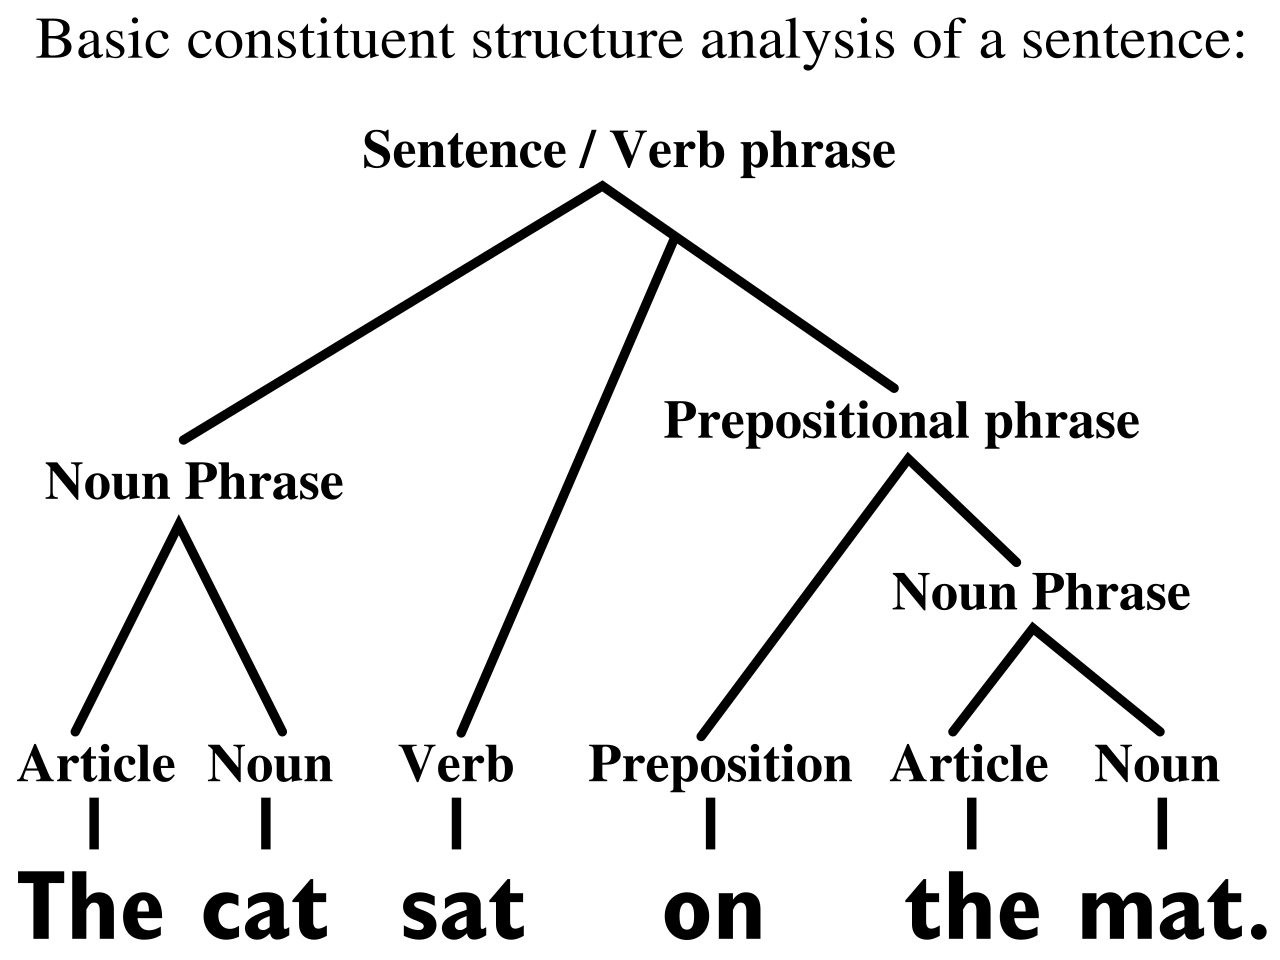
\includegraphics[width=0.82\linewidth]{assets/images/zpracovani-textovych-dat/syntax-tree.png}
  \caption[Syntaktický strom věty]{Příklad konstituentního syntaktického stromu. Popis obrázku: věta je
  rozložena na jmennou frázi, slovesnou část a předložkovou frázi; strom ukazuje hierarchii částí věty,
  kterou lze využít při parsingu nebo extrakci vztahů. Zdroj obrázku: AnonMoos,
  \href{https://commons.wikimedia.org/wiki/File:Basic\_constituent\_structure\_analysis\_English\_sentence.svg}{Wikimedia
  Commons}, public domain.}
  \label{fig:q18-syntax-tree}
\end{figure}

\subsection{Coreference resolution}

Coreference resolution řeší, které výrazy odkazují na stejnou entitu.

Příklad:
\begin{quote}
\uv{Koupil jsem telefon Samsung. Je velmi rychlý.}
\end{quote}

Zájmeno \uv{Je} odkazuje na:
\[
\text{telefon Samsung}.
\]

Coreference je důležitá pro:
\begin{itemize}
    \item extrakci informací,
    \item sumarizaci,
    \item sentiment,
    \item otázky a odpovědi.
\end{itemize}

\subsection{Reprezentace textu pro modely}

Algoritmy obvykle neumějí pracovat přímo s textem. Potřebují číselnou reprezentaci:
\[
\text{text}
\rightarrow
\mathbf{x}\in\mathbb{R}^p.
\]

Základní přístupy:
\begin{itemize}
    \item bag-of-words,
    \item n-gramy,
    \item TF-IDF,
    \item topic modely,
    \item word embeddings,
    \item contextual embeddings,
    \item sentence embeddings.
\end{itemize}

\subsection{Bag-of-words}

Bag-of-words reprezentuje dokument podle výskytu slov bez ohledu na jejich pořadí.

Dokument:
\[
d_i=(w_{i1},w_{i2},\ldots,w_{ip}),
\]
kde $p$ je velikost slovníku.

Hodnota $w_{ij}$ může být:
\begin{itemize}
    \item binární výskyt,
    \item četnost termu,
    \item TF-IDF váha.
\end{itemize}

Výhody:
\begin{itemize}
    \item jednoduché,
    \item dobře použitelné s klasickými ML modely,
    \item interpretovatelné.
\end{itemize}

Nevýhody:
\begin{itemize}
    \item ztrácí pořadí slov,
    \item nezachycuje význam,
    \item má vysokou dimenzi,
    \item nezvládá dobře synonymii a polysémii.
\end{itemize}

\subsection{N-gramy}

N-gram je posloupnost $n$ tokenů:
\[
(w_t,w_{t+1},\ldots,w_{t+n-1}).
\]

Příklady:
\begin{itemize}
    \item unigram: \texttt{data},
    \item bigram: \texttt{data mining},
    \item trigram: \texttt{natural language processing}.
\end{itemize}

N-gramy zachytí část lokálního pořadí slov. Jsou užitečné například pro:
\begin{itemize}
    \item klasifikaci textů,
    \item jazykové modely,
    \item vyhledávání frází,
    \item detekci ustálených spojení.
\end{itemize}

Nevýhoda:
\begin{itemize}
    \item velikost slovníku rychle roste s $n$.
\end{itemize}

\subsection{TF-IDF reprezentace}

TF-IDF váha:
\[
w_{ij}
=
tf_{ij}\cdot idf_j.
\]

Kde:
\[
idf_j=
\log\left(\frac{N}{df_j}\right).
\]

TF-IDF zvýrazňuje slova, která jsou častá v daném dokumentu, ale vzácná v celé kolekci.

Použití:
\begin{itemize}
    \item vyhledávání,
    \item klasifikace dokumentů,
    \item clustering dokumentů,
    \item podobnost dokumentů.
\end{itemize}

Kosinová podobnost:
\[
\cos(d_i,d_j)
=
\frac{d_i^\top d_j}
{\|d_i\|\|d_j\|}.
\]

\subsection{Klasické jazykové modely}

Jazykový model přiřazuje pravděpodobnost posloupnosti slov:
\[
P(w_1,w_2,\ldots,w_T).
\]

Pomocí řetězového pravidla:
\[
P(w_1,\ldots,w_T)
=
\prod_{t=1}^{T}
P(w_t|w_1,\ldots,w_{t-1}).
\]

Protože dlouhá historie je nepraktická, n-gramový model zjednodušuje:
\[
P(w_t|w_1,\ldots,w_{t-1})
\approx
P(w_t|w_{t-n+1},\ldots,w_{t-1}).
\]

Bigramový model:
\[
P(w_1,\ldots,w_T)
\approx
\prod_{t=1}^{T}
P(w_t|w_{t-1}).
\]

Problém:
\begin{itemize}
    \item mnoho n-gramů se ve vzorku nevyskytne,
    \item potřebujeme vyhlazování,
    \item model má omezený kontext,
    \item nepracuje dobře se synonymy ani s významem.
\end{itemize}

\subsection{Word embeddings}

Word embedding je vektorová reprezentace slova:
\[
w
\mapsto
\mathbf{e}_w\in\mathbb{R}^k.
\]

Na rozdíl od one-hot reprezentace je embedding:
\begin{itemize}
    \item hustý,
    \item nízkorozměrný,
    \item naučený z dat,
    \item schopný zachytit významovou podobnost.
\end{itemize}

One-hot reprezentace:
\[
\text{pes}=(0,0,1,0,\ldots,0).
\]

Embedding:
\[
\text{pes}\mapsto (0.12,-0.41,0.33,\ldots).
\]

Podobnost slov lze měřit kosinovou podobností:
\[
\cos(\mathbf{e}_a,\mathbf{e}_b)
=
\frac{\mathbf{e}_a^\top\mathbf{e}_b}
{\|\mathbf{e}_a\|\|\mathbf{e}_b\|}.
\]

\subsection{Distribuční hypotéza}

Embeddingy vycházejí z distribuční hypotézy:
\begin{center}
slova s podobným kontextem mají podobný význam.
\end{center}

Například slova \uv{pes} a \uv{kočka} se často vyskytují v podobných kontextech:
\begin{center}
\uv{krmit}, \uv{zvíře}, \uv{mazlíček}, \uv{veterinář}.
\end{center}

Proto by jejich vektory měly být blízko.

\subsection{Word2Vec}

Word2Vec je metoda pro učení slovních embeddingů pomocí jednoduché neuronové sítě.

Existují dvě základní varianty:
\begin{itemize}
    \item \textbf{CBOW} -- z kontextu predikuje prostřední slovo;
    \item \textbf{Skip-gram} -- z prostředního slova predikuje okolní slova.
\end{itemize}

\begin{figure}[htbp]
  \centering
  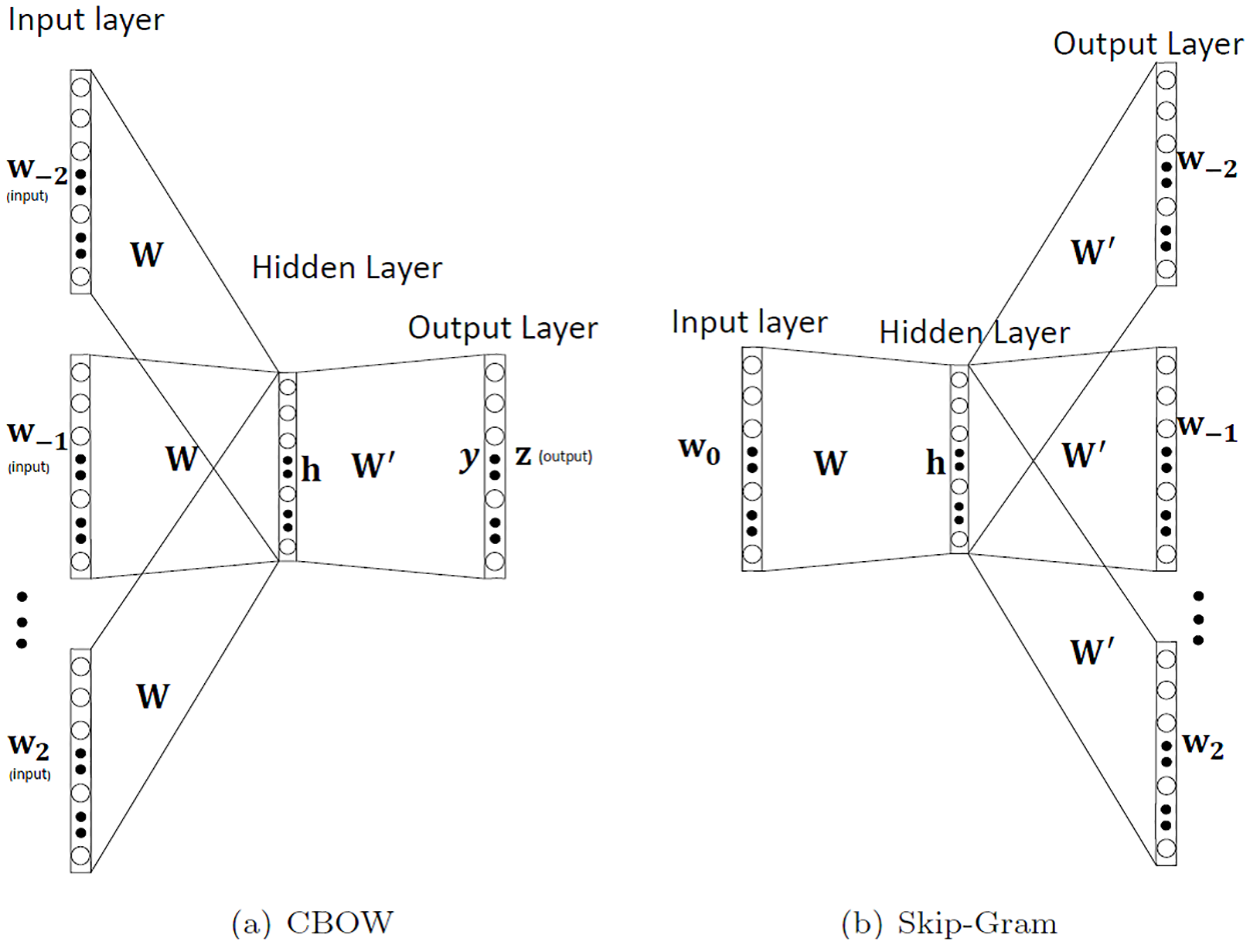
\includegraphics[width=0.92\linewidth]{assets/images/zpracovani-textovych-dat/word2vec-cbow-skipgram.png}
  \caption[CBOW a Skip-gram ve Word2Vec]{Dvě varianty architektury Word2Vec. Popis obrázku: CBOW na levé
  straně používá okolní slova k predikci prostředního slova, zatímco Skip-gram na pravé straně používá
  prostřední slovo k predikci jeho okolního kontextu. Zdroj obrázku: Kimothi, Biyani, Hogan, Soni, Kelly,
  \href{https://doi.org/10.1371/journal.pone.0216636.g001}{PLOS ONE / Figshare}, licence CC BY 4.0.}
  \label{fig:q18-word2vec}
\end{figure}

\subsubsection{CBOW}

CBOW:
\[
(w_{t-r},\ldots,w_{t-1},w_{t+1},\ldots,w_{t+r})
\rightarrow
w_t.
\]

Model dostane okolní slova a snaží se odhadnout slovo uprostřed.

Vlastnosti:
\begin{itemize}
    \item rychlejší trénování,
    \item dobré pro častá slova.
\end{itemize}

\subsubsection{Skip-gram}

Skip-gram:
\[
w_t
\rightarrow
(w_{t-r},\ldots,w_{t-1},w_{t+1},\ldots,w_{t+r}).
\]

Model dostane slovo a snaží se odhadnout jeho kontext.

Vlastnosti:
\begin{itemize}
    \item lepší pro méně častá slova,
    \item potřebuje méně dat pro zachycení vzácnějších vztahů,
    \item často používá negative sampling pro zrychlení trénování.
\end{itemize}

\subsection{GloVe}

GloVe je metoda založená na matici spoluvýskytů slov. Využívá globální informaci o tom, která slova se
vyskytují ve stejných kontextech.

Obecná idea:
\[
X_{ij}
=
\operatorname{cooc}(i,j).
\]

GloVe hledá vektory, které dobře vysvětlují poměry spoluvýskytů.

\subsection{Omezení klasických embeddingů}

Word2Vec a GloVe jsou typicky \textbf{context-free}. Každé slovo má jeden vektor bez ohledu na význam.

Problém:
\[
\text{bank}
\]
může znamenat:
\begin{itemize}
    \item finanční instituci,
    \item břeh řeky.
\end{itemize}

Context-free embedding má pro oba významy jeden vektor.

\subsection{Kontextové embeddingy a transformery}

Moderní modely jako BERT nebo GPT vytvářejí kontextové reprezentace. Stejné slovo může mít různý vektor
podle věty.

\[
\text{bank}_{\text{finance}}
\neq
\text{bank}_{\text{river}}.
\]

Transformer používá mechanismus attention:
\[
Attention(Q,K,V)
=
softmax
\left(
\frac{QK^\top}{\sqrt{d_k}}
\right)V.
\]

\paragraph{Intuice.}
Každý token se \uv{dívá} na jiné tokeny ve větě a určuje, které jsou pro jeho interpretaci důležité.

\begin{figure}[htbp]
  \centering
  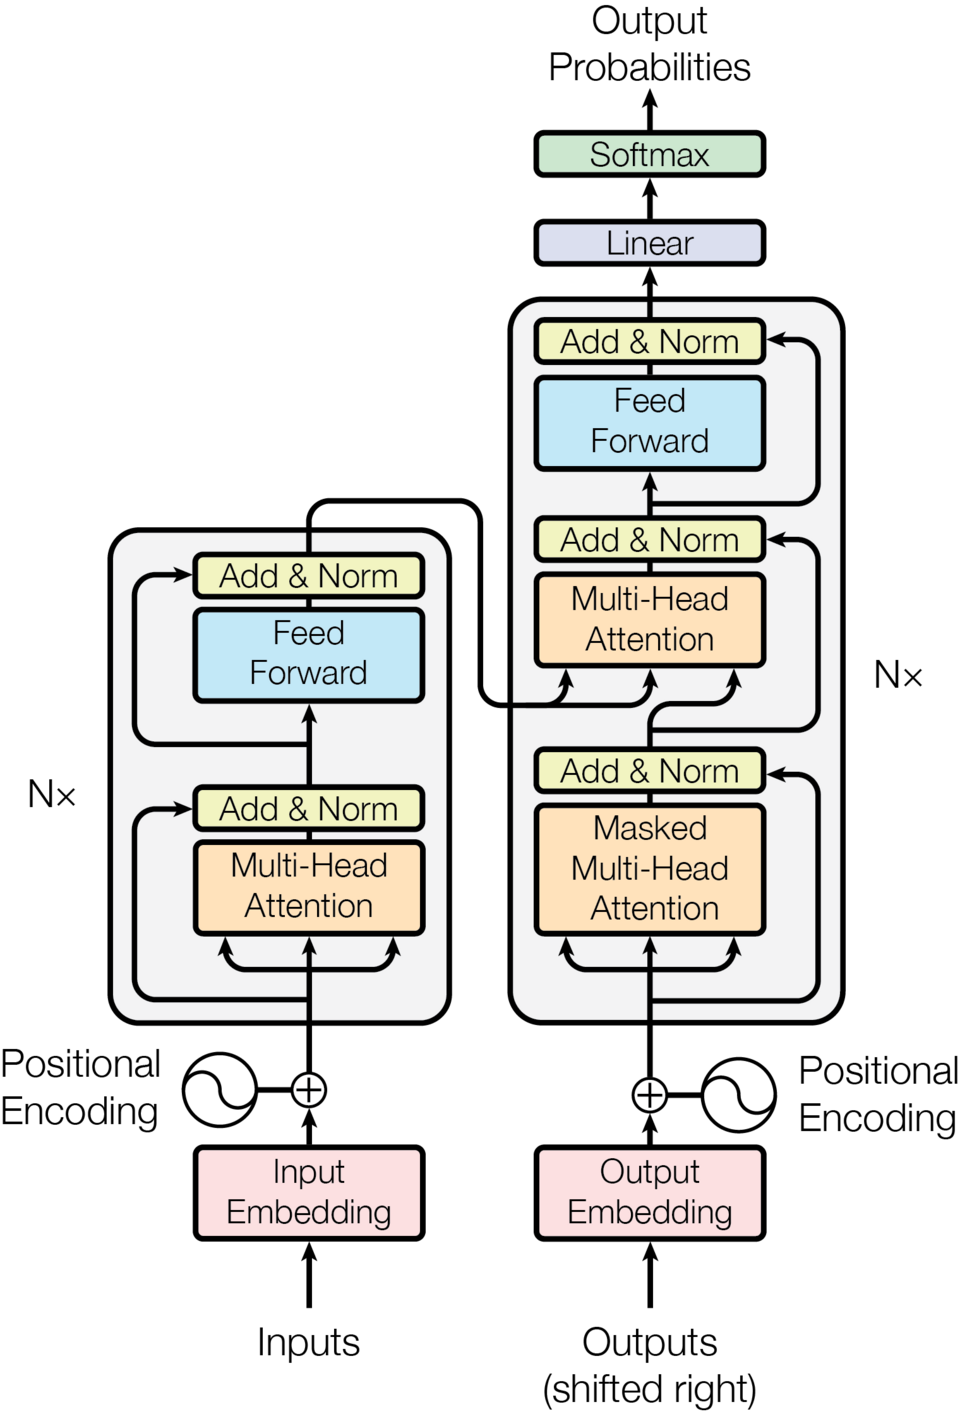
\includegraphics[width=0.54\linewidth]{assets/images/zpracovani-textovych-dat/transformer-architecture.png}
  \caption[Architektura transformeru]{Architektura encoder-decoder transformeru. Popis obrázku: vstupní a
  výstupní tokeny se převádějí na embeddingy s pozičním kódováním, procházejí bloky multi-head attention,
  feed-forward vrstvami a normalizacemi; decoder navíc používá maskovanou attention pro autoregresivní
  generování. Zdroj obrázku: Google,
  \href{https://commons.wikimedia.org/wiki/File:Attention\_Is\_All\_You\_Need\_-\_Encoder-decoder\_Architecture.png}{Wikimedia
  Commons}, licence CC BY-SA 4.0.}
  \label{fig:q18-transformer}
\end{figure}

\subsection{Typy jazykových modelů}

\begin{itemize}
    \item \textbf{N-gramové modely} -- pravděpodobnost dalšího slova podle krátké historie.
    
    \item \textbf{Word2Vec / GloVe} -- učí vektorové reprezentace slov.
    
    \item \textbf{Encoder-only transformery} -- například BERT; vhodné pro klasifikaci, NER a porozumění textu.
    
    \item \textbf{Decoder-only transformery} -- například GPT; vhodné pro generování textu.
    
    \item \textbf{Encoder-decoder transformery} -- vhodné pro překlad, sumarizaci a převod jedné sekvence na jinou.
    
    \item \textbf{Sentence embeddings} -- například Sentence-BERT; vhodné pro podobnost vět, sémantické vyhledávání
    a clustering dokumentů.
\end{itemize}

\subsection{Analytické metody nad textem}

\subsubsection{Textová klasifikace}

Textová klasifikace přiřazuje dokumentu třídu:
\[
d_i \rightarrow y_i.
\]

Příklady:
\begin{itemize}
    \item spam / ne-spam,
    \item téma článku,
    \item typ zákaznického požadavku,
    \item pozitivní / negativní sentiment,
    \item rizikový / nerizikový dokument.
\end{itemize}

Modely:
\begin{itemize}
    \item Naive Bayes,
    \item logistická regrese,
    \item SVM,
    \item rozhodovací stromy,
    \item random forest,
    \item gradient boosting,
    \item neuronové sítě,
    \item transformery.
\end{itemize}

Vyhodnocení:
\[
Accuracy,\quad Precision,\quad Recall,\quad F_1.
\]

\subsubsection{Clustering dokumentů}

Clustering hledá skupiny podobných dokumentů bez předem známých tříd.

Postup:
\begin{enumerate}
    \item reprezentovat dokumenty jako TF-IDF nebo embeddingy,
    \item spočítat podobnosti,
    \item použít shlukovací algoritmus,
    \item interpretovat shluky podle nejtypičtějších slov nebo dokumentů.
\end{enumerate}

Použitelné algoritmy:
\begin{itemize}
    \item k-means,
    \item hierarchické shlukování,
    \item DBSCAN,
    \item HDBSCAN.
\end{itemize}

\subsubsection{Topic modeling}

Topic modeling hledá skrytá témata v kolekci dokumentů.

Základní idea:
\[
\text{document}
=
\text{mixture of topics},
\]
\[
\text{topic}
=
\text{distribution over words}.
\]

LDA modeluje:
\[
P(w|d)
=
\sum_{k=1}^{K}
P(w|z=k)P(z=k|d).
\]

Kde:
\begin{itemize}
    \item $z$ je latentní téma,
    \item $P(w|z)$ říká, která slova jsou typická pro téma,
    \item $P(z|d)$ říká, jaká témata jsou zastoupena v dokumentu.
\end{itemize}

\begin{figure}[htbp]
  \centering
  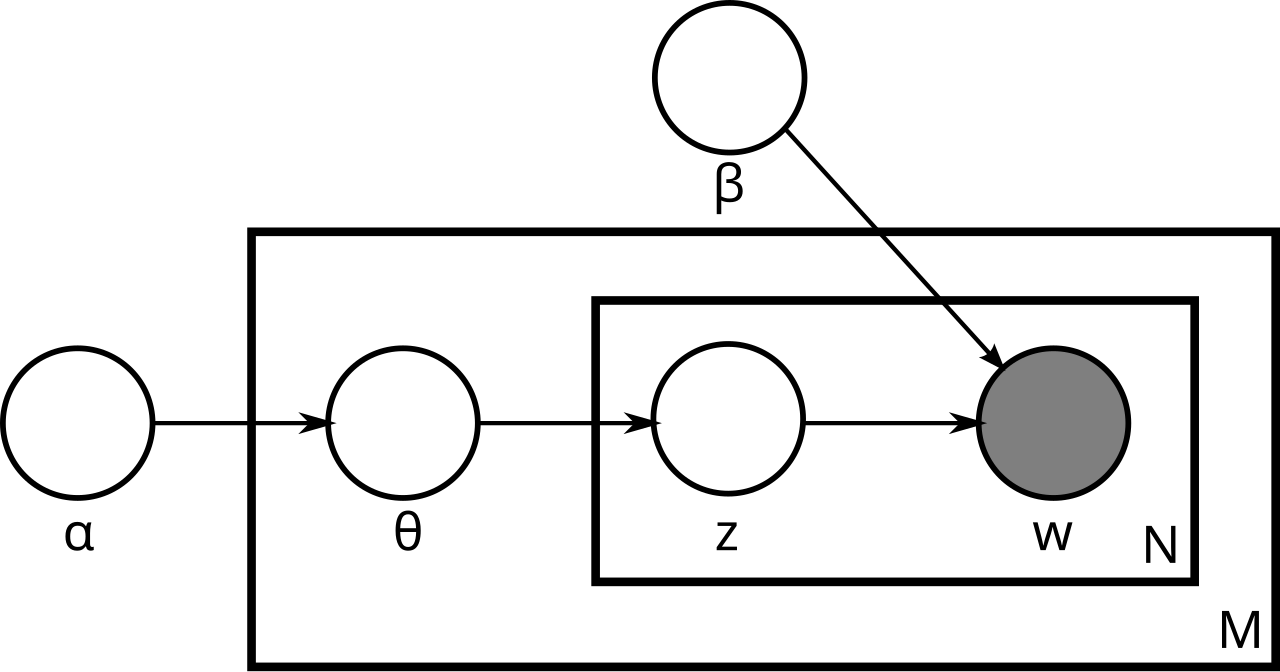
\includegraphics[width=0.78\linewidth]{assets/images/zpracovani-textovych-dat/lda-plate-notation.png}
  \caption[LDA v plate notation]{Grafický model Latent Dirichlet Allocation v plate notation. Popis obrázku:
  dokument má rozdělení témat $\theta$, každé slovo má latentní téma $z$ a pozorované slovo $w$; opakování
  přes slova a dokumenty je vyznačeno obdélníky. Zdroj obrázku: Bkkbrad,
  \href{https://commons.wikimedia.org/wiki/File:Latent\_Dirichlet\_allocation.svg}{Wikimedia Commons},
  licence CC BY-SA 4.0.}
  \label{fig:q18-lda}
\end{figure}

Použití:
\begin{itemize}
    \item explorace velké kolekce textů,
    \item monitoring médií,
    \item analýza zákaznické zpětné vazby,
    \item tematická segmentace dokumentů.
\end{itemize}

\subsubsection{Named Entity Recognition}

NER hledá pojmenované entity:
\[
\text{Oliver Blume} \rightarrow PERSON,
\]
\[
\text{Volkswagen} \rightarrow ORGANIZATION,
\]
\[
\text{23 MEUR} \rightarrow MONEY.
\]

Přístupy:
\begin{itemize}
    \item regulární výrazy,
    \item gazetteery,
    \item pravidla,
    \item CRF,
    \item transformerové modely,
    \item LLM.
\end{itemize}

Vyhodnocení NER:
\[
Precision=
\frac{TP}{TP+FP},
\qquad
Recall=
\frac{TP}{TP+FN},
\qquad
F_1=
2\frac{PR}{P+R}.
\]

Rozlišuje se:
\begin{itemize}
    \item \textbf{strict match} -- přesně stejný rozsah entity i typ,
    \item \textbf{relaxed match} -- částečná shoda rozsahu nebo tolerantnější hodnocení.
\end{itemize}

\subsubsection{Relation extraction}

Relation extraction hledá vztahy mezi entitami:
\[
relation(e_1,e_2).
\]

Příklad:
\[
CEO\_of(\text{Oliver Blume},\text{Volkswagen}).
\]

Přístupy:
\begin{itemize}
    \item pravidlové vzory,
    \item dependency parsing,
    \item supervised learning,
    \item distant supervision,
    \item transformerové modely,
    \item LLM s následnou validací.
\end{itemize}

\subsection{Sentiment analysis}

Sentiment analysis neboli opinion mining se zabývá zjišťováním názorů, postojů, hodnocení a sentimentu
vyjádřeného v textu.

Typické třídy:
\[
positive,\quad negative,\quad neutral.
\]

Sentiment lze analyzovat na různých úrovních:
\begin{itemize}
    \item \textbf{document-level} -- sentiment celého dokumentu;
    \item \textbf{sentence-level} -- sentiment věty;
    \item \textbf{aspect-based} -- sentiment ke konkrétnímu aspektu entity.
\end{itemize}

\subsubsection{Opinion quintuple}

Formální reprezentace názoru:
\[
(e_j,a_{jk},so_{ijkl},h_i,t_l).
\]

Kde:
\begin{itemize}
    \item $e_j$ je cílová entita,
    \item $a_{jk}$ je aspekt entity,
    \item $so_{ijkl}$ je sentimentová hodnota,
    \item $h_i$ je držitel názoru,
    \item $t_l$ je čas vyjádření názoru.
\end{itemize}

Příklad:
\[
(\text{iPhone},\ \text{battery life},\ -,\ \text{user123},\ \text{2025-01-10}).
\]

\subsubsection{Sentimentové lexikony}

Lexikonový přístup používá seznamy slov s polaritou:
\[
\text{good} \rightarrow +,
\qquad
\text{bad} \rightarrow -.
\]

Problémy:
\begin{itemize}
    \item význam závisí na doméně,
    \item slova mohou být ironická,
    \item sentiment může být vyjádřen faktem,
    \item nutné řešit negaci a modifikátory.
\end{itemize}

\subsubsection{Shifters a modifikátory polarity}

Negace:
\[
\text{good}
\rightarrow +,
\qquad
\text{not good}
\rightarrow -.
\]

Zesilovače:
\[
\text{very good}
\]
znamená silnější pozitivní sentiment.

Zeslabovače:
\[
\text{slightly bad}
\]
znamená slabší negativní sentiment.

Adverzativní spojky:
\[
\text{A, but B}
\]
často zvyšují význam části za \uv{but}.

\paragraph{Problém ironie.}
Věta:
\begin{quote}
\uv{Skvělé, aplikace zase spadla.}
\end{quote}
obsahuje pozitivní slovo \uv{skvělé}, ale celkový sentiment je negativní.

\subsection{Sumarizace textu}

Sumarizace převádí dlouhý text nebo kolekci textů na kratší přehled.

Typy:
\begin{itemize}
    \item \textbf{extraktivní sumarizace} -- vybírá důležité věty z původního textu;
    \item \textbf{abstraktivní sumarizace} -- generuje nové formulace.
\end{itemize}

Použití:
\begin{itemize}
    \item shrnutí dokumentů,
    \item shrnutí recenzí,
    \item shrnutí reportů,
    \item monitoring médií.
\end{itemize}

U názorů je často důležitá \textbf{aspect-based sumarizace}, například:
\begin{center}
60 \% uživatelů chválí fotoaparát, 40 \% kritizuje baterii.
\end{center}

\subsection{Question answering a RAG}

Předtrénované jazykové modely mají omezení:
\begin{itemize}
    \item nemusí obsahovat nejnovější informace,
    \item mohou halucinovat,
    \item slabě pokrývají úzké domény,
    \item neumí vždy spolehlivě uvést zdroje,
    \item výstup může být příliš obecný.
\end{itemize}

Retrieval-Augmented Generation, RAG, kombinuje jazykový model s vyhledáváním.

Postup:
\[
\begin{aligned}
\text{query}
&\rightarrow
\text{retrieval}
\rightarrow
\text{relevant passages},\\
\text{query + passages}
&\rightarrow
\text{prompt augmentation}
\rightarrow
\text{generation}.
\end{aligned}
\]

\begin{figure}[htbp]
  \centering
  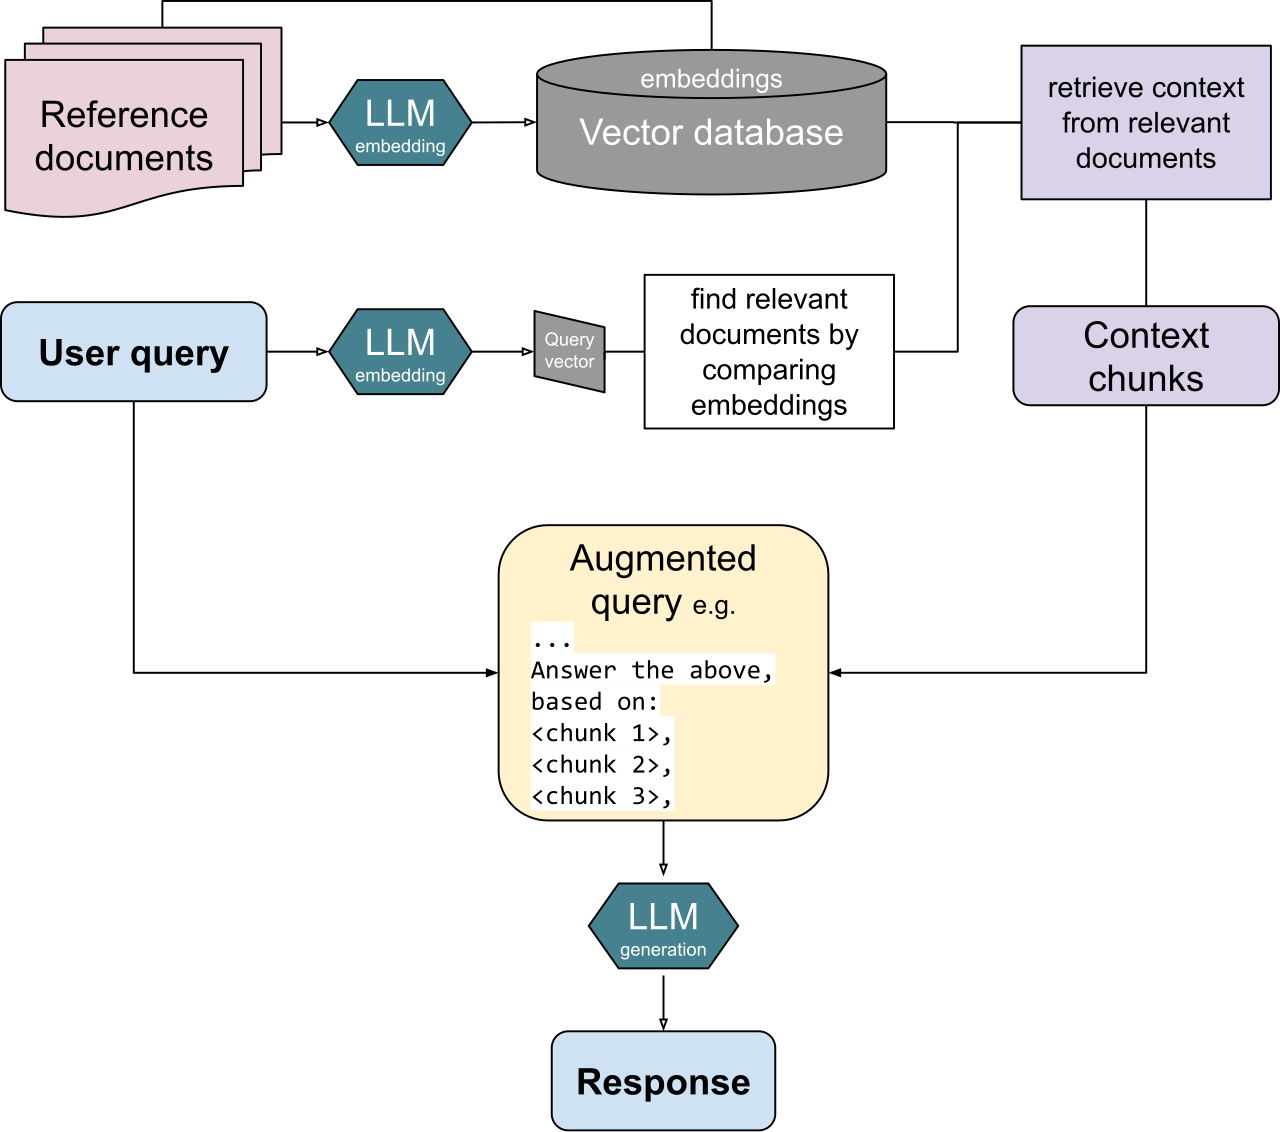
\includegraphics[width=0.82\linewidth]{assets/images/zpracovani-textovych-dat/rag-diagram.png}
  \caption[Retrieval-Augmented Generation]{Zjednodušené schéma RAG. Popis obrázku: referenční dokumenty se
  převedou na embeddingy a uloží do vektorové databáze; dotaz uživatele se také převede na vektor, podle
  podobnosti se vyhledají relevantní části dokumentů a ty se spolu s dotazem vloží do promptu pro jazykový
  model. Zdroj obrázku: Turtlecrown,
  \href{https://commons.wikimedia.org/wiki/File:RAG\_diagram.svg}{Wikimedia Commons}, licence CC BY-SA 4.0.}
  \label{fig:q18-rag}
\end{figure}

RAG umožňuje využít:
\begin{itemize}
    \item novější texty,
    \item doménově specifické dokumenty,
    \item kurátorsky ověřené zdroje,
    \item lokální firemní dokumentaci.
\end{itemize}

\subsubsection{Sparse a dense retrieval v RAG}

Sparse retrieval:
\[
TF\text{-}IDF,\quad BM25.
\]

Dense retrieval:
\[
\text{Sentence-BERT embeddings},\quad \text{vector database}.
\]

Dense retrieval je vhodný pro sémantickou podobnost, sparse retrieval je často lepší pro přesná klíčová
slova, kódy a názvy.

\subsection{Knowledge graphs a KG-RAG}

Znalostní graf ukládá fakta jako uzly a hrany:
\[
(entity_1) \xrightarrow{relation} (entity_2).
\]

Příklad:
\[
(\text{Volkswagen}) \xrightarrow{CEO} (\text{Oliver Blume}).
\]

KG-RAG využívá místo nebo vedle textového korpusu strukturovaný znalostní graf. Výhody:
\begin{itemize}
    \item přesnější a kurátorovanější fakta,
    \item lepší vysvětlitelnost,
    \item možnost grafového dotazování,
    \item menší riziko halucinací než u volného textu.
\end{itemize}

\subsection{Vyhodnocení textových metod}

\subsubsection{Klasifikace}

\[
Accuracy=
\frac{TP+TN}{TP+TN+FP+FN}.
\]

\[
Precision=
\frac{TP}{TP+FP}.
\]

\[
Recall=
\frac{TP}{TP+FN}.
\]

\[
F_1=
2\frac{Precision\cdot Recall}{Precision+Recall}.
\]

\subsubsection{IR}

U vyhledávání:
\begin{itemize}
    \item precision@k,
    \item recall@k,
    \item MAP,
    \item NDCG,
    \item MRR.
\end{itemize}

Precision@k:
\[
Precision@k
=
\frac{\#\text{ relevant documents in top } k}
{k}.
\]

\subsubsection{NER a IE}

U NER:
\begin{itemize}
    \item strict span match,
    \item relaxed span match,
    \item micro/macro precision, recall, F1.
\end{itemize}

U relation extraction:
\begin{itemize}
    \item správnost dvojice entit,
    \item správnost typu vztahu,
    \item správnost celého trojčlenu.
\end{itemize}

\subsubsection{Sumarizace a generování}

Používají se automatické metriky:
\begin{itemize}
    \item ROUGE,
    \item BLEU,
    \item BERTScore.
\end{itemize}

U generativních modelů je však často nutné lidské hodnocení:
\begin{itemize}
    \item věcná správnost,
    \item úplnost,
    \item čitelnost,
    \item relevance,
    \item citace zdrojů,
    \item bezpečnost.
\end{itemize}

\subsection{Existující nástroje}

\subsubsection{Python}

\begin{itemize}
    \item \texttt{re} -- regulární výrazy;
    \item \texttt{pandas} -- práce s tabulkovými výstupy;
    \item \texttt{scikit-learn} -- TF-IDF, klasifikace, clustering;
    \item \texttt{NLTK} -- základní NLP a výuka;
    \item \texttt{spaCy} -- tokenizace, POS tagging, NER, dependency parsing;
    \item \texttt{Stanza} -- NLP pipeline od Stanford NLP;
    \item \texttt{UDPipe} -- tokenizace, lemmatizace, POS tagging a parsing, vhodné i pro češtinu;
    \item \texttt{Gensim} -- Word2Vec, topic modeling;
    \item \texttt{transformers} -- modely BERT, GPT a další;
    \item \texttt{sentence-transformers} -- sentence embeddings;
    \item \texttt{Haystack}, \texttt{LangChain}, \texttt{LlamaIndex} -- RAG aplikace.
\end{itemize}

\subsubsection{R}

\begin{itemize}
    \item \texttt{tidytext},
    \item \texttt{quanteda},
    \item \texttt{tm},
    \item \texttt{text2vec},
    \item \texttt{udpipe},
    \item \texttt{stm}.
\end{itemize}

\subsubsection{Vyhledávání a indexace}

\begin{itemize}
    \item Apache Lucene,
    \item Elasticsearch,
    \item OpenSearch,
    \item Solr,
    \item FAISS,
    \item Milvus,
    \item Pinecone,
    \item Weaviate,
    \item Chroma.
\end{itemize}

Lucene/Elasticsearch jsou typické pro sparse retrieval a fulltextové vyhledávání. FAISS a vektorové
databáze jsou typické pro dense retrieval nad embeddingy.

\subsubsection{Anotace dat}

\begin{itemize}
    \item doccano,
    \item Label Studio,
    \item Prodigy,
    \item brat,
    \item INCEpTION,
    \item GATE.
\end{itemize}

Anotace je důležitá pro supervised úlohy jako sentiment, NER, relation extraction nebo klasifikace dokumentů.

\subsection{Typické problémy při zpracování textu}

\begin{itemize}
    \item mnoho jazykových variant,
    \item překlepy a neformální jazyk,
    \item ironie a sarkasmus,
    \item doménová specifika,
    \item nejednoznačnost slov,
    \item coreference,
    \item nedostatek anotovaných dat,
    \item nevyvážené třídy,
    \item změna témat v čase,
    \item bias v datech,
    \item ochrana osobních údajů.
\end{itemize}

\subsection{Tradiční NLP vs. deep learning}

\subsubsection{Tradiční přístup}

Tradiční NLP často používá:
\begin{itemize}
    \item ruční nebo lingvistické příznaky,
    \item tokenizaci,
    \item lemmatizaci,
    \item POS tagging,
    \item syntaktické příznaky,
    \item TF-IDF,
    \item klasické ML modely.
\end{itemize}

Výhody:
\begin{itemize}
    \item lepší interpretovatelnost,
    \item nižší výpočetní náklady,
    \item použitelné na menších datech.
\end{itemize}

Nevýhody:
\begin{itemize}
    \item vyžaduje feature engineering,
    \item hůře zachycuje hlubší význam,
    \item často horší výkon u složitých úloh.
\end{itemize}

\subsubsection{Deep learning přístup}

Moderní modely, hlavně transformery, pracují více end-to-end:
\[
\text{text}
\rightarrow
\text{tokenizer}
\rightarrow
\text{transformer}
\rightarrow
\text{output}.
\]

Výhody:
\begin{itemize}
    \item vysoký výkon,
    \item kontextové reprezentace,
    \item transfer learning,
    \item méně ručního feature engineeringu.
\end{itemize}

Nevýhody:
\begin{itemize}
    \item vyšší nároky na výpočetní výkon,
    \item horší interpretovatelnost,
    \item riziko halucinací u generativních modelů,
    \item potřeba kontroly biasu a bezpečnosti.
\end{itemize}

\subsection{Doporučený praktický postup}

\begin{enumerate}
    \item definovat úlohu: klasifikace, vyhledávání, extrakce, sumarizace;
    \item zkontrolovat zdroj a kvalitu dat;
    \item vyčistit a normalizovat text;
    \item vytvořit vhodnou reprezentaci textu;
    \item zvolit baseline model, například TF-IDF + logistická regrese;
    \item porovnat s pokročilejší metodou, například embeddingy nebo transformer;
    \item vyhodnotit na oddělených datech;
    \item analyzovat chyby;
    \item ošetřit právní, etické a bezpečnostní aspekty;
    \item připravit nasazení a monitoring.
\end{enumerate}

\subsection{Shrnutí ke zkoušce}

Zpracování textových dat převádí přirozený jazyk do podoby vhodné pro vyhledávání, modelování a extrakci
informací. Základní NLP pipeline zahrnuje tokenizaci, rozdělení vět, normalizaci, lemmatizaci, POS tagging,
syntaktické zpracování, NER, relation extraction a coreference resolution.

Text lze reprezentovat klasicky pomocí bag-of-words, n-gramů a TF-IDF:
\[
w_{ij}=tf_{ij}\cdot idf_j,
\]
nebo moderně pomocí embeddingů:
\[
w \mapsto \mathbf{e}_w\in\mathbb{R}^k.
\]

Word2Vec využívá CBOW nebo Skip-gram a učí slovní vektory z kontextu. Moderní transformery vytvářejí
kontextové reprezentace a jsou základem současných jazykových modelů. RAG kombinuje vyhledávání dokumentů
s generováním odpovědi:
\[
Retrieval \rightarrow Augmentation \rightarrow Generation.
\]

Mezi hlavní analytické metody patří klasifikace textu, sentiment analysis, topic modeling, clustering,
NER, relation extraction, sumarizace, question answering a sémantické vyhledávání. Prakticky se používají
nástroje jako Python knihovny scikit-learn, spaCy, Gensim, transformers a sentence-transformers,
vyhledávací systémy Elasticsearch a FAISS, R balíčky tidytext a quanteda nebo anotovací nástroje doccano
a Label Studio.

\subsection{Zdroje}

\begin{itemize}
    \item Jurafsky, Martin:
    \href{https://web.stanford.edu/~jurafsky/slp3/ed3book.pdf}{Speech and Language Processing}.
    \item spaCy dokumentace:
    \href{https://spacy.io/usage/linguistic-features}{Linguistic Features}.
    \item scikit-learn dokumentace:
    \href{https://scikit-learn.org/stable/modules/feature\_extraction.html\#text-feature-extraction}{Text
    feature extraction}.
    \item Gensim dokumentace:
    \href{https://radimrehurek.com/gensim/models/word2vec.html}{Word2Vec}.
    \item Vaswani et al.:
    \href{https://arxiv.org/abs/1706.03762}{Attention Is All You Need}.
    \item Lewis et al.:
    \href{https://arxiv.org/abs/2005.11401}{Retrieval-Augmented Generation for Knowledge-Intensive NLP Tasks}.
    \item Blei, Ng, Jordan:
    \href{https://www.jmlr.org/papers/v3/blei03a.html}{Latent Dirichlet Allocation}.
    \item Bing Liu:
    \href{https://www.cs.uic.edu/~liub/FBS/SentimentAnalysis-and-OpinionMining.pdf}{Sentiment Analysis and
    Opinion Mining}.
    \item Wikimedia Commons:
    \href{https://commons.wikimedia.org/wiki/File:Basic\_constituent\_structure\_analysis\_English\_sentence.svg}{Basic
    constituent structure analysis English sentence}.
    \item PLOS ONE / Figshare:
    \href{https://doi.org/10.1371/journal.pone.0216636.g001}{Word2Vec architecture}.
    \item Wikimedia Commons:
    \href{https://commons.wikimedia.org/wiki/File:Attention\_Is\_All\_You\_Need\_-\_Encoder-decoder\_Architecture.png}{Attention
    Is All You Need -- Encoder-decoder Architecture}.
    \item Wikimedia Commons:
    \href{https://commons.wikimedia.org/wiki/File:Latent\_Dirichlet\_allocation.svg}{Latent Dirichlet allocation}.
    \item Wikimedia Commons:
    \href{https://commons.wikimedia.org/wiki/File:RAG\_diagram.svg}{RAG diagram}.
\end{itemize}

\newpage
